\documentclass{beamer} 
\usetheme{default} 
\usecolortheme{albatross}
\setbeamercovered{transparent}
%\useoutertheme{umbcfootline}  


\usepackage[spanish]{babel}
%\usepackage[latin1]{inputenc}
\usepackage[utf8x]{inputenc}
\usepackage{hyperref}
\usepackage{color}



\usepackage{multicol}


\title{HERENCIA}

\author{Manuel J. Molino Milla \and Luis Molina Garzón}

\date{\today} %

\institute{IES Virgen del Carmen \and Departamento de Informática}




%\beamerdefaultoverlayspecification{<+->}

\begin{document}


\begin{frame}
  \titlepage
\end{frame}

\begin{frame}
    \frametitle{Logo}
\begin{figure}

\includegraphics[scale=1]{imagenes/logo.jpeg} 
\caption{Logo Java}
\end{figure}
\end{frame}

\begin{frame}
  \frametitle{Contenido}
  \tableofcontents[pausesections]
\end{frame}



\section{Herencia}

\begin{frame}
\frametitle{Introduccion a la herencia}
\begin{itemize}[<+->]
\item Una de las características de la \emph{POO} es que unas clases deriven de otras.
\item A esta característica se le donomina \alert{herencia}
\item De esa manera aumentamos la potencialidad del código la hacerlo mas \emph{reusable}
\item Ejmplo: podemos definir clase de cuerpo geométricos: Círculo, Triangulo, Cuadrado, Rectángulo, \dots
\item Pero todas ellas tienen características comunes, como número de lados, área, perímetro, \dots.
\item Los que nos permitiría crear una clase base, por ejemplo \emph{CuerposGeometricos} y obtener el resto por herencia.
\item Así un cuadrado determinado es un objeto de la clase Cuadrado y también, a su vez por herencia, es un CuerpoGeometrico.
\end{itemize}
\end{frame}

\begin{frame}
\frametitle{Herencia}
\begin{itemize}[<+->]
\item Siempre se está haciendo herencia, pues todas las clases derivan de la clase \textbf{Object}
\item Para decir que una clase hereda de otra, usamos la palabra reservada \alert{extends}
\item \emph{public class ClaseHija extends ClasePadre}
\item Solamente puede haber una clase padre, es decir después de \emph{extends} solo puede aparacer una sola clase.
\item Java no permite \emph{herencia múltiple} como ocurre en \emph{C++}
\item A la clase padre también se le llama \emph{superclase} o \emph{clase base}
\item A la clase hija también se le denomina \emph{clase derivada}, \emph{clase extendida} o \emph{subclase}.
\item Una clase hija hereda todos los atributos y métodos accesibles de la clase padre.
\item Además podrá añadir nuevos atributos y métodos.
\item \textbf{No podrá acceder a atributos y métodos privados de la superclase.}
\end{itemize}
\end{frame}

\begin{frame}
\frametitle{Palabra reservada super}
\begin{itemize}[<+->]
\item Una subclase puede llamar al constructor de la clase padre.
\item Para esto usamos la palabra clave \alert{super}.
\item Para hacer esto usamos: \textbf{super()}
\item O bién para llamer a métodos de la clase padre:
\item \textbf{super.metodoDeLaSuperClase(parámetros)}
\end{itemize} 
\end{frame}

\begin{frame}
\frametitle{UML herencia}
\begin{figure}
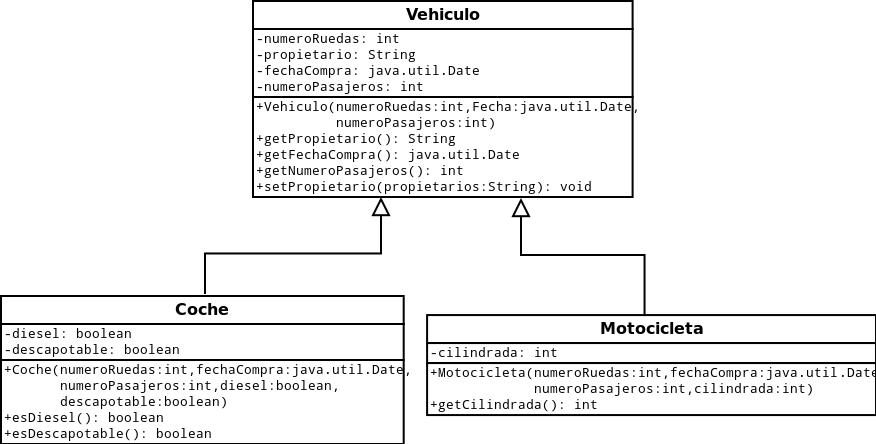
\includegraphics[scale=0.35]{imagenes/uml.png}
\end{figure}
\end{frame}


\begin{frame}[fragile]
\frametitle{Clase padre} 
\begin{tiny}
\begin{verbatim}
public class Vehiculo
{
  private int numeroRuedas;
  private String propietario;
  private java.util.Date fechaCompra;
  private int numeroPasajeros;
  public Vehiculo (int numeroRuedas, java.util.Date fechaCompra,
                   int numeroPasajeros)
  {
    this.numeroRuedas = numeroRuedas;
    this.fechaCompra = fechaCompra;
    this.numeroPasajeros = numeroPasajeros;
  }
  public String getPropietario ()
  {
    return this.propietario;
  }
  public java.util.Date getFechaCompra ()
  {
    return this.fechaCompra;
  }
  public int getNumeroPasajeros ()
  {
    return numeroPasajeros;
  }
  public void setPropietario (String propietario)
  {
    this.propietario = propietario;
  }
}
\end{verbatim}
\end{tiny}
\end{frame}


\begin{frame}[fragile]
    \frametitle{Clases hijas}
\begin{tiny}
\begin{multicols}{2}
\begin{verbatim}
public class Motocicleta extends Vehiculo
{
  private int cilindrada;
  public Motocicleta (
    int numeroRuedas, java.util.Date fechaCompra,
    int numeroPasajeros, int cilindrada)
  {
    super (numeroRuedas, fechaCompra,
           numeroPasajeros);
    this.cilindrada = cilindrada;
  }
  public int getCilindrada ()
  {
    return this.cilindrada;
  }
}

\end{verbatim}
\begin{verbatim}
public class Coche extends Vehiculo{
  private boolean diesel;
  private boolean descapotable;
  public Coche (int numeroRuedas, 
         java.util.Date fechaCompra,
         int numeroPasajeros, boolean diesel, 
         boolean descapotable){
    super (numeroRuedas, fechaCompra, numeroPasajeros);
    this.diesel = diesel;
    this.descapotable = descapotable;
  }
  public boolean esDiesel (){
    return this.diesel;
  }
  public boolean esDescapotable (){
    return this.descapotable;
  }
}
\end{verbatim}
\end{multicols}
\end{tiny}
\end{frame}


\begin{frame}[fragile]
    \frametitle{Llamada a los constructores}
  \begin{itemize}[<+->]
\item Un constructor de una clase derivada puede invocar al constructor de la clase superior con \textbf{super} o incluso puede sobregarcarglo.
\item Ademas si no se llama a ningun constructor de la superclase con \emph{super} el lo invoca de todas formas.
\item Ejemplo:
 \end{itemize}
 \pause
 \begin{figure}
 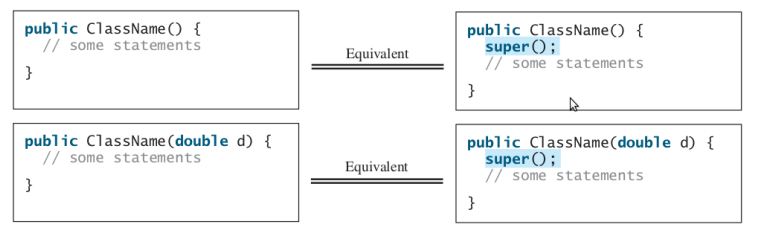
\includegraphics[scale=0.4]{imagenes/constructor.png}
 \end{figure}
 \pause
 Siempre que se crea una instancia de la subclase se crea una instancia de la superclase.
\end{frame}




\begin{frame}[fragile]
    \frametitle{¿Cual es la salida de este codigo?}
    \begin{multicols}{2}
\begin{tiny}
\begin{verbatim}
public class Uno extends Dos
{
  public static void main (String[]args)
  {
    new Uno ();
  }
  public Uno ()
  {
    System.out.println ("Constructor de uno");
  }
}

class Dos extends Tres
{
  public Dos ()
  {
    this ("Llamando al constructor de Dos");
    System.out.println ("Constructor de Dos");
  }
  public Dos (String s)
  {
    System.out.println (s);
  }
}

class Tres
{
  public Tres ()
  {
    System.out.println ("Constructor de Tres");
  }
}
\end{verbatim}
\end{tiny}
\end{multicols}
\pause
\begin{footnotesize}
\begin{verbatim}
Constructor de Tres
Llamando al constructor de Dos
Constructor de Dos
Constructor de uno
\end{verbatim}
\end{footnotesize}
\end{frame}

\begin{frame}[fragile]
    \frametitle{Sobrescribir métodos}
   \begin{itemize}[<+->]
   \item Una subclase hereda los métodos de la superclase.
   \item A veces, para la subclase, es necesario cambiar la implementación de un método definido en la superclase.
   \item Hablamos de sobrescribir métodos.
   \item Ejemplo, el método \textbf{toString()}, que se hereda directamente de la clase ráiz, \emph{Object}
   \item Donde podemos mostrar las caracteristicas del objeto segun nos interese.
   \item No debemos olvidar que NO podemos sobrescribir \emph{métodos privados}
   \item Los métodos estáticos pueden heredarse a las clases hijas.
   
   \end{itemize}
\end{frame}


\begin{frame}[fragile]
\frametitle{Ejemplo}
\framesubtitle{¿Cuál método está sobrescrito y cuál sobrecargado?}
\begin{center}
\alert{¿Qué muestran por pantalla esto dos programas?}
\end{center}
\begin{tiny}
\begin{multicols}{2}
\begin{verbatim}
public class Test1 { 
 public static void main(String[] args) { 
  A a = new A(); 
  a.p(10); 
  a.p(10.0); 
 } 
}
class B { 
 public void p(double i) { 
  System.out.println(i * 2); 
 } 
}
class A extends B { 
 public void p(double i ) { 
  System.out.println(i); 
 } 
}

public class Test2 {
 public static void main(String[] args) {
  A a = new A();
  a.p(10);
  a.p(10.0);
 }
}
class B {
 public void p(double i) {
  System.out.println(i * 2);
 }
}
class A extends B {
 public void p(int i ) {
  System.out.println(i);
 }
}
\end{verbatim}
\end{multicols}
\end{tiny}
\pause
\begin{center}
\alert{En el primero se sobrescribe y en el segundo se sobrecarga.}\\
\pause
\alert{El primero da 10.0 10.0 y el segundo 10 20.0}
\end{center}
\end{frame}




\begin{frame}[fragile]
    \frametitle{Otros Ejemplo}
    \framesubtitle{¿Es correcto este código?}
   \begin{scriptsize}
\begin{verbatim}
public class Estatica1
{
  static int valor = 0;
  public static void incrementar ()
  {
    valor += 1;
  }
}
class Estatica2 extends Estatica1
{
  public static void incrementar ()
  {
    valor += 2;
  }
  public static void main (String[]arg)
  {
    Estatica1.incrementar ();
    incrementar ();
    System.out.println (valor);
  }
}
\end{verbatim} 
\pause
\begin{center}
\alert{La salida es 3. Se sobrescribe el metodo estatico}\\
\pause
\alert{Se puede llamar al metodo de la superclase con \emph{Superclase.Metodo}}
\end{center}
\end{scriptsize}

\end{frame}


\begin{frame}
    \frametitle{Clase Object}
\begin{footnotesize}
\begin{itemize}[<+->]
\item La clase Object, en el paquete java.lang, se sitúa en la parte más alta del árbol de jerarquía.
\item Cada clase es un descendiente, directo o indirecto, de la clase Object.
\item Cada clase que usa o escribe hereda los métodos de instancia de Object.
\item No necesita usar ninguno de estos métodos, pero, si podemos sobrecargarlos.
\item Entre ellos estan:
\begin{enumerate}
\item \alert{protected Object clone() throws CloneNotSupportedException}  Crea y devuelve una copia de este objeto.
\item \alert{public boolean equals(Object obj)} indica si dos objetos son idénticos.
\item \alert{protected void finalize() throws Throwable} Llamado por el recolector cuando ya no hay más referencias al objeto 
\item \alert{public final Class getClass()} Devuelve la clase de tiempo de ejecución de un objeto.
\item \alert{public int hashCode()} Devuelve un valor identificador para el objeto.
\item \alert{public String toString()} Devuelve una representación de cadena del objeto.
\end{enumerate}
\end{itemize}
\end{footnotesize}

\end{frame}



\begin{frame}[fragile]
\frametitle{Metodo equals}
El método \alert{equals} de la clase Object compara las referencias de los objetos. Pero se puede sobrescribir para que actúe a nuestro gusto:
\pause
\begin{verbatim}
public class Persona {
  private String nombre;
  private LocalDate fechaNacimiento;
  private String dni;
	
  public Persona(String nombre, 
    LocalDate fechaNacimiento, String dni) {
      this.nombre = nombre;
      this.fechaNacimiento = fechaNacimiento;
      this.dni = dni;
  }
  ...............	
}
\end{verbatim}
\pause
¿Cómo se sobreescribe el método equals? Dos personas son iguales si tienen la misma fecha de nacimiento y dni.
\end{frame}


\begin{frame}[fragile]
\frametitle{Metodo equals}
\begin{footnotesize}
\begin{verbatim}
@Override
 public boolean equals(Object obj) {
  if (this == obj)
    return true;
  if (obj == null)
    return false;
  if (getClass() != obj.getClass())
    return false;
  Persona other = (Persona) obj;
  if (dni == null) {
    if (other.dni != null)
      return false;
  } else if (!dni.equals(other.dni))
    return false;
  if (fechaNacimiento == null) {
    if (other.fechaNacimiento != null)
      return false;
  } else if (!fechaNacimiento.equals(other.fechaNacimiento))
    return false;
  return true;
 }
\end{verbatim}
\end{footnotesize}
\end{frame}

\begin{frame}[fragile]
\frametitle{Metodo equals}
Usando el método \emph{equals} de la clase \emph{Objects}
\begin{verbatim}
@Override
  public boolean equals(Object obj) {
    if (this == obj)
      return true;
    if (obj == null)
      return false;
    if (getClass() != obj.getClass())
      return false;
    Persona other = (Persona) obj;
      return Objects.equals(this.dni,  other.dni) &&
         Objects.equals(this.dni, other.fechaNacimiento);
  }
\end{verbatim}
\end{frame}

\begin{frame}[fragile]
\frametitle{Metodo toString}
El método toString() de Object devuelve una representación  String del objeto, que es muy útil para la depuración. Pero también se puede sobrescribir.
\begin{tiny}
\begin{verbatim}
public class ClasePrincipal1
{
  private int id;
  private String nombre;
  public ClasePrincipal1 (int id, String nombre)
  {
    this.id = id;
    this.nombre = nombre;
  }
//sobrescribimos el método toString
  public String toString ()
  {
    String s = this.id + "-" + this.nombre;
    return s;
  }
  public static void main (String[]arg)
  {
    ClasePrincipal1 p1 = new ClasePrincipal1 (1, "uno");
    ClasePrincipal1 p2 = new ClasePrincipal1 (1, "one");
    System.out.println (p1.toString ());
    System.out.println (p2.toString ());
  }
}
\end{verbatim}
\end{tiny}
\pause
\begin{center}
La sálida es: \alert{1-uno 1-one}
\end{center}

\end{frame}


\begin{frame}[fragile]
\begin{tiny}
\frametitle{Método clone}
\begin{itemize}[<+-|alert@+>]
\item En algunas situaciones deseamos que un objeto que se pasa a una función, o bien, que un objeto que llama a una función miembro no se modifiquen en el curso de la llamada.
\item  Por ejemplo, un objeto de la clase Lista al llamar a la función miembro ordenar modifica la posición de los datos en el array.
\item Sería por tanto mantener una copia del objeto original.
\item La clase base Object de todas las clases en el lenguaje Java, tiene una función miembro denominada clone, que se redefine en la clase derivada para realizar una duplicación de un objeto de dicha clase.  
\item Para esto se ha de implementar el interface Cloneable.
\item Ademas se ha de redefinir la función miembro clone de la clase base Object
\end{itemize}
\pause
\begin{verbatim}
public class Persona implements Cloneable{
    private String nombre;
    private int edad;
    ...
    public Object clone(){
        Object obj=null;
        try{
            obj=super.clone();
        }catch(CloneNotSupportedException ex){
            System.out.println("No se puede duplicar");
        }
        return obj;
    }
    ....
}
\end{verbatim}
\pause
\begin{verbatim}
Persona p =  new Persona("Manuel", 35); //objeto original
Persona pCopia = (Persona)p.clone(); //objeto copia
\end{verbatim}
\end{tiny}
\end{frame}


\begin{frame}[fragile]
\frametitle{Metodo finalize}
\begin{itemize}[<+->]
\item Antes de que \emph{recolector de basura actúe}.
\item JVM puede usar el método \emph{finalize}
\item Que permita a JVM liberar recursos del sistema, como archivos abiertos o sockets abiertos antes de actuar \emph{garbage collected}.
\end{itemize}
\pause
\begin{scriptsize}
\begin{verbatim}
class OpenAFile {
    FileInputStream aFile = null;
    OpenAFile(String filename) {
        try {
            aFile = new FileInputStream(filename);
        } catch (java.io.FileNotFoundException e) {
            System.err.println("Could not open file " + filename);
        }
    }
    .....
    protected void finalize () throws throwable {
    if (aFile != null) {
        aFile.close();
        aFile = null;
    }
    ....
}
}

\end{verbatim}
\end{scriptsize}
\end{frame}

\begin{frame}
\frametitle{Acceso protected}
\begin{description}[<+->]
\item[public] Todos los miembros públicos pueden ser accedidos desde otra clase sin restrinción alguna.
\item[private] Todo lo contrario, no pueden se accedidos. Se suele usar los \emph{getters} y \emph{setters} para acceder a ellos, siempre y cuando, estos últimos sean públicos.
\item[amistoso] Acceso a nivel de paquete.
\item[protected] Sólamente son accesible desde las subclases.
\end{description}
\begin{figure}
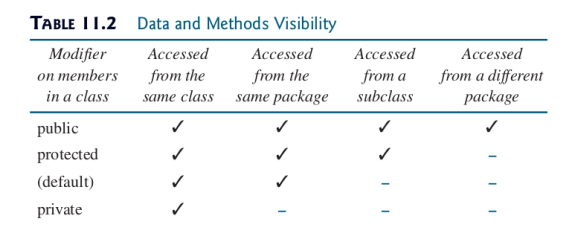
\includegraphics[scale=0.5]{imagenes/acceso.png}
\end{figure}
\end{frame}

\begin{frame}
\frametitle{Ejemplo} 
\begin{figure}
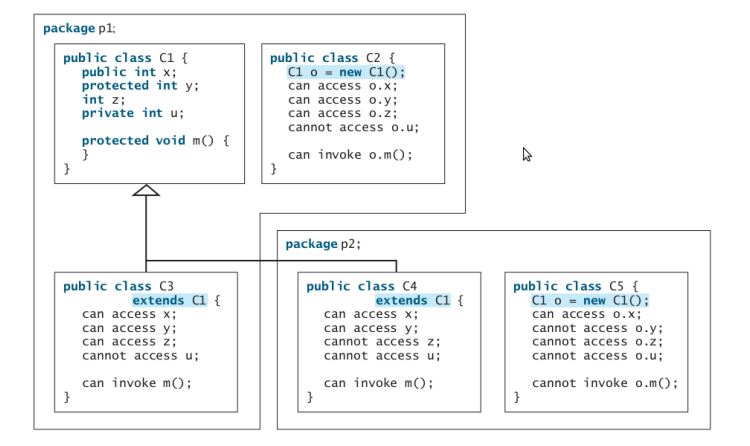
\includegraphics[scale=0.5]{imagenes/ejemplo.png} 
\end{figure} 
\end{frame}

\begin{frame}[fragile]
\frametitle{Clase final}
\begin{itemize}[<+->]
\item Podemos diseñar una clase en la que NO se puedan diseñar subclases.
\item En estos casos usamos el modificador \textbf{final} para indicar que es una clase final y no es padre de ninguna otra.
\item Ejemplo de clases finales: \emph{Math, String, StringBuilder, \dots}
\item Ejemplo:
\end{itemize}
\pause
\begin{verbatim}
public final class SeAcabo{
...
}
\end{verbatim}
\pause
\begin{itemize}[<+->]
\item Los métodos también pueden ser finales.
\item Eso implica que no pueden ser sobrescritos. 
\end{itemize}
\pause
\begin{small}
\begin{verbatim}
public class Test {
   ...
   public final void m() {
   ...
   }
}
\end{verbatim}
\end{small}


\end{frame}


\begin{frame}[fragile]
\frametitle{Ejemplo}
\begin{itemize}[<+->]
\item Los modificadores SOLO se pueden usar en clases y miembros de clase.
\item EXCEPTO el modificador final que también se puede usar en variables de métodos locales.
\item Una variable final declarada en un método se considera una constante en ese método.
\item Ejemplo:
\end{itemize}
\pause
\begin{small}
\begin{verbatim}
public class Ejemplo{
  public int variable1;
  private int variable2;
  protected int variable3;
  final int VARIABLE4=6; //hay que inicializar

  public void metodoEjemplo(){
    final int VARIABLE5= 5; //posible
//    public int variable6; //MAL
//    private int variable7;//MAL
  }
}
\end{verbatim}
\end{small}
\end{frame}

\begin{frame}
\frametitle{Preguntas} 
\begin{figure}

\includegraphics[scale=0.9]{imagenes/dudas.png}
\end{figure} 
\end{frame}

\end{document}

